
\begin{figure} \begin{center}
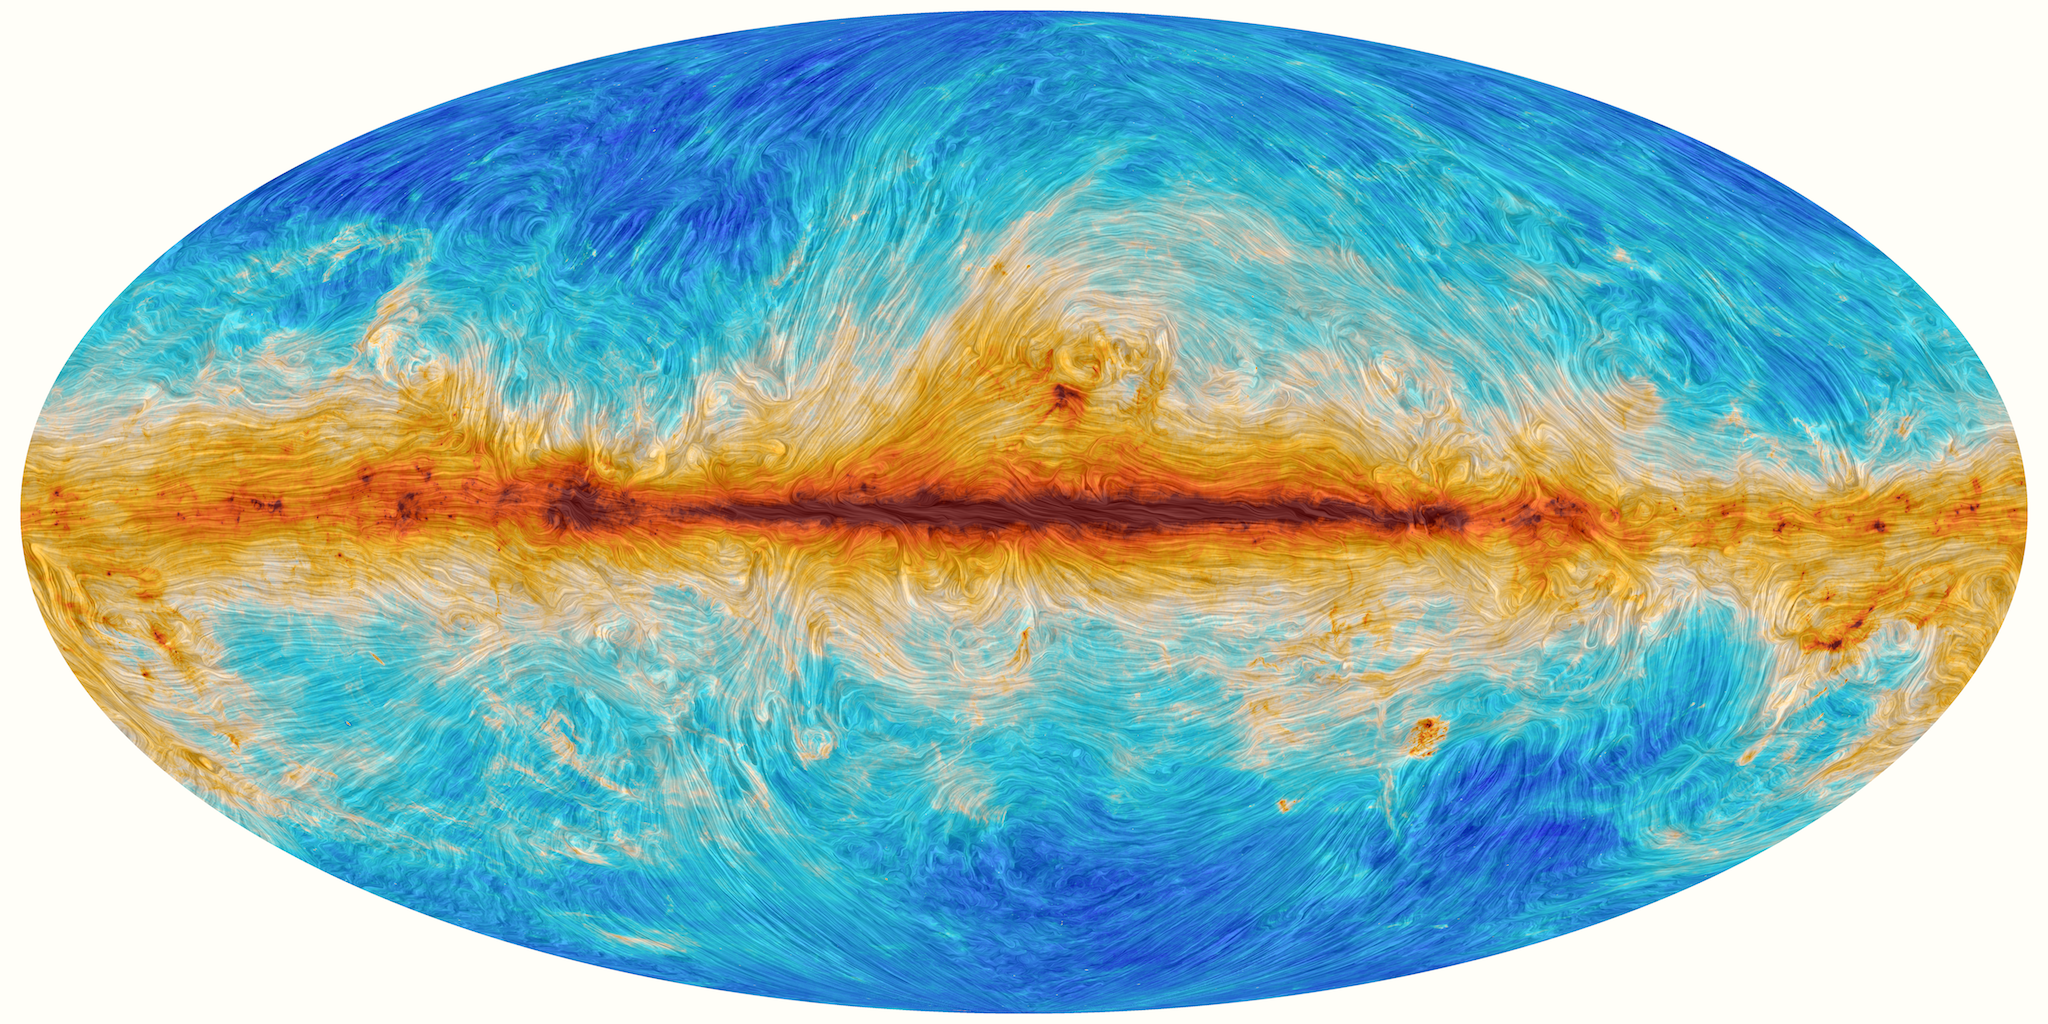
\includegraphics[width=0.55\textwidth]{figs/2015_353GHz_B-field.png}
%\includegraphics[width=0.42\textwidth]{figs/ClEE_y_12panel_average.pdf}
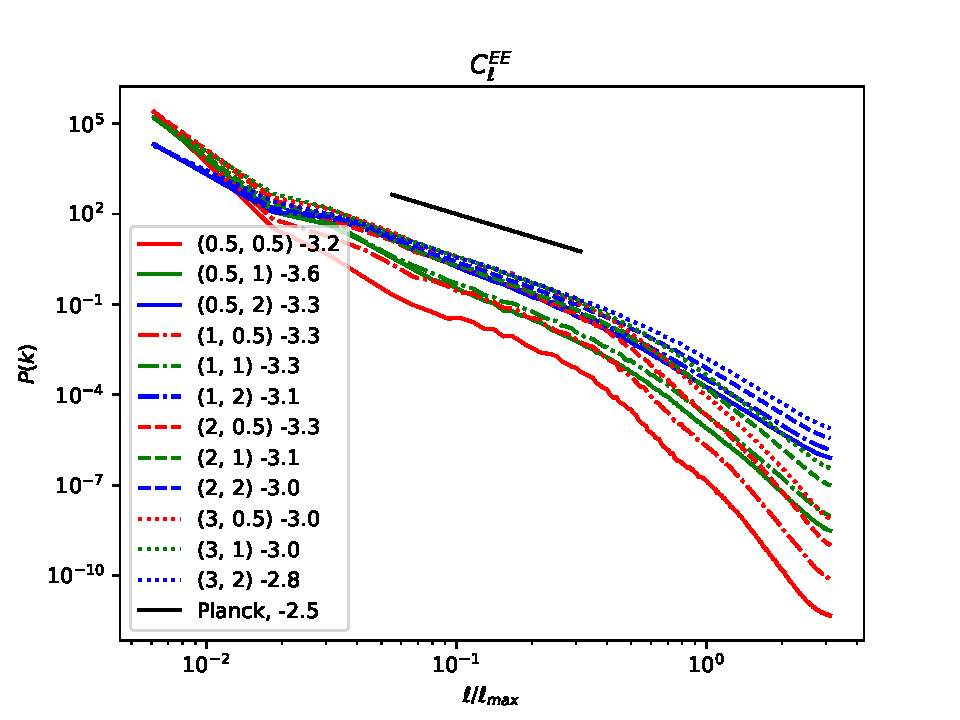
\includegraphics[width=0.42\textwidth]{figs/alpha_TEB.pdf}
\caption[ ]{\emph{(Left)} The large scale magnetic field of the galaxy as seen by the Planck
satellite. The color field shows dust emission at 353GHz.  The image is smeared
along the direction of the magnetic field \citep{PlanckXIX15}.  The \nameCMB\
project aims to understand the observational properties of this signal, while the \nameGalaxies\
project aims to understand its origin. \emph{(Right)} The power spectrum of the
polarization showing $E-$mode power vs. wavenumber for a preliminary suite of
simulations (colored lines) and the galaxy (black line).}
\label{fig.planck} \end{center} \end{figure}
